%%%%%%%%%%%%%%%%%%%%%%%%%%%%%%%%%%%%%%%%%%%%%%%%%%%%%%%%%%%%%%%%%%%%%
% This is a LaTeX template for students
% working on Homework 6, Computer Architecture I, Spring, 2022.
% You SHALL NOT distribute this template.
%%%%%%%%%%%%%%%%%%%%%%%%%%%%%%%%%%%%%%%%%%%%%%%%%%%%%%%%%%%%%%%%%%%%%
\section{Shut Up and Take My Cache!}
In this section, we will review some basics of cache. A program is
run on a byte-addressed system with a single-level cache. After a
while, the entire cache has the state in Figure \ref{fig:layout}.

\begin{figure}[h]
    \centering
    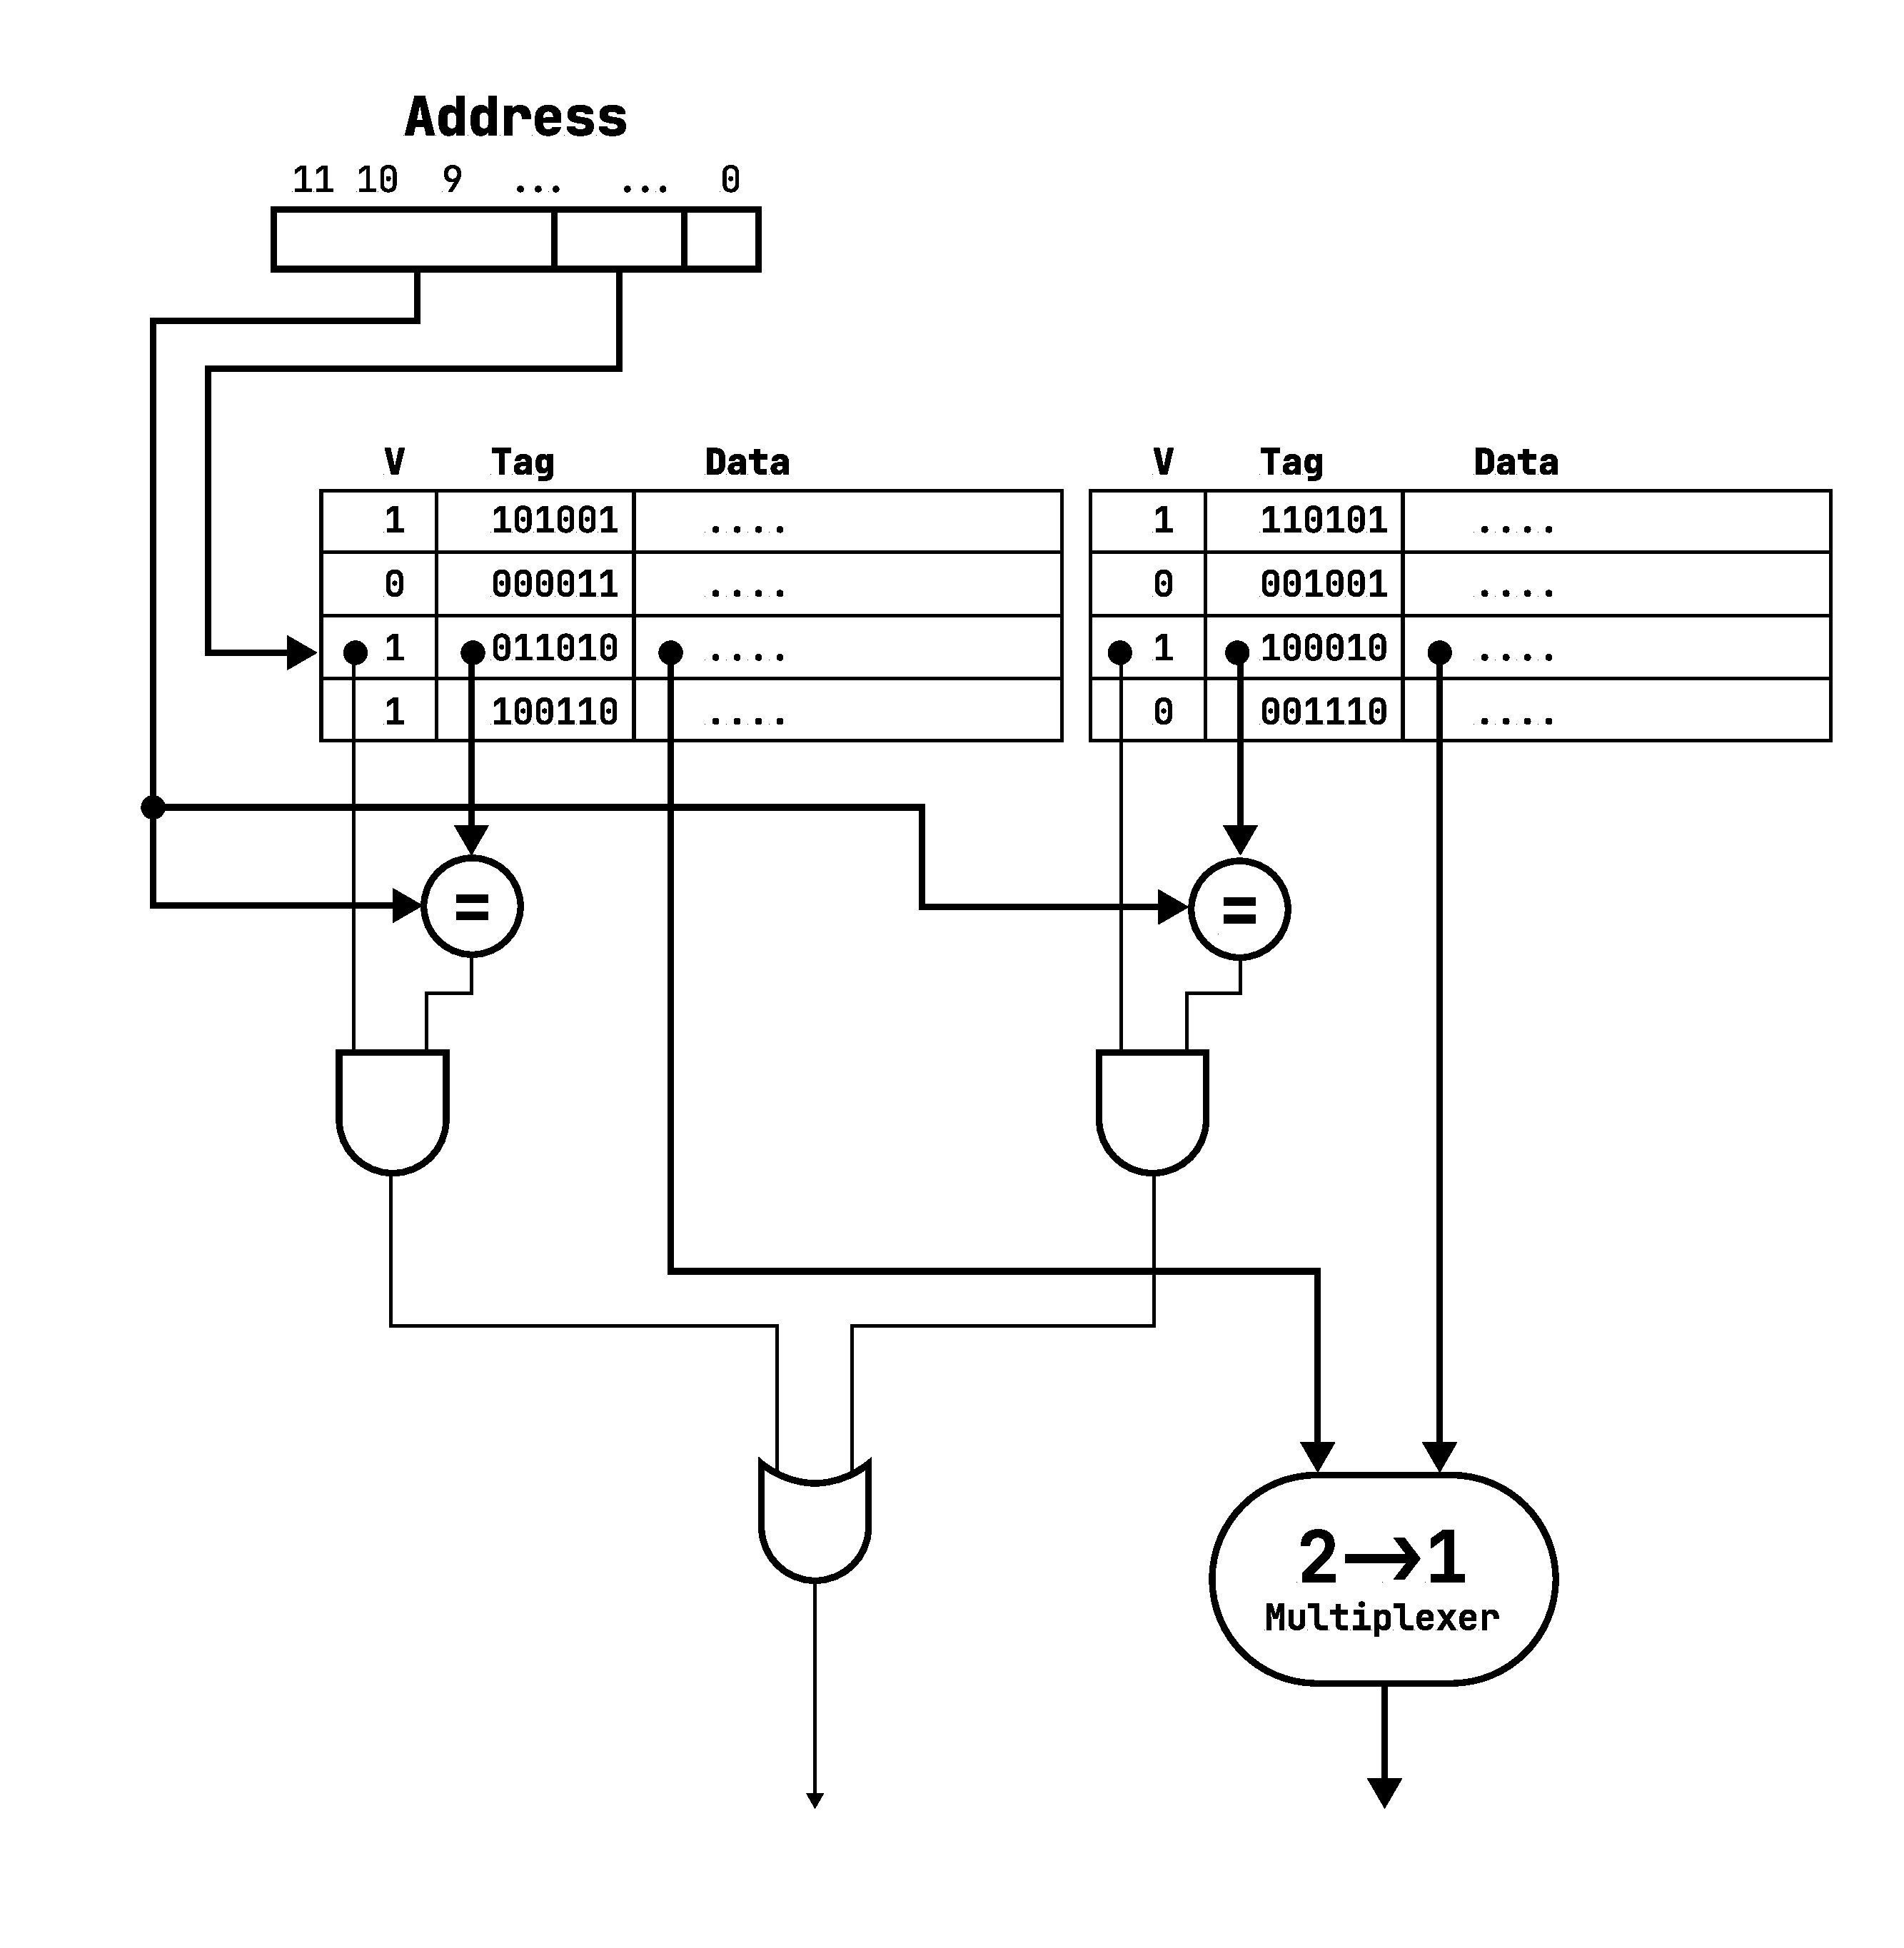
\includegraphics[width=0.9\textwidth]{img/layout.pdf}
    \caption{Layout for a cache implementation}
    \label{fig:layout}
\end{figure}

\newpage

\begin{questions}

\question[2] In Figure \ref{fig:layout}, what is a row stands for?
{

    \begin{oneparchoices}
        \choice One set.
        \choice One cache block.
        \choice One entire cache.
        \choice Not listed in choices.
    \end{oneparchoices}
    
    \begin{solution}
        \begin{oneparcheckboxes}
            %%%%%%%%%%% YOUR ANSWER HERE %%%%%%%%%%%%%%%%%%%%%%%%%%%%
            % If you find the correct answer, substitute `\choice` by
            % `\CorrectChoice`!
            %%%%%%%%%%%%%%%%%%%%%%%%%%%%%%%%%%%%%%%%%%%%%%%%%%%%%%%%%
            \CorrectChoice A
            \choice B
            \choice C
            \choice D
        \end{oneparcheckboxes}
    \end{solution}

}

\question[2] In Figure \ref{fig:layout}, what is \texttt{V} stands
for?
{

    \begin{oneparchoices}
        \choice Valid bit.
        \choice Vacant bit.
        \choice Visited bit.
    \end{oneparchoices}
    
    \begin{solution}
        \begin{oneparcheckboxes}
            %%%%%%%%%%% YOUR ANSWER HERE %%%%%%%%%%%%%%%%%%%%%%%%%%%%
            % If you find the correct answer, substitute `\choice` by
            % `\CorrectChoice`!
            %%%%%%%%%%%%%%%%%%%%%%%%%%%%%%%%%%%%%%%%%%%%%%%%%%%%%%%%%
            \CorrectChoice A
            \choice B
            \choice C
        \end{oneparcheckboxes}
    \end{solution}

}

\question[2] What is the type of the cache described in Figure \ref{fig:layout}?
{

    \begin{choices}
        \choice Direct-Mapped cache.
        \choice Set-Associative Cache (If you choose this, write
        down its associativity).
        \choice Fully-Associative Cache (If you choose this, write
        down its associativity).
    \end{choices}
    
    \begin{solution}
        \begin{checkboxes}
            %%%%%%%%%%% YOUR ANSWER HERE %%%%%%%%%%%%%%%%%%%%%%%%%%%%
            % If you find the correct answer, substitute `\choice` by
            % `\CorrectChoice`!
            % If you choose B or C, write your answer in `\fillin[]`
            % arguments.
            %%%%%%%%%%%%%%%%%%%%%%%%%%%%%%%%%%%%%%%%%%%%%%%%%%%%%%%%%
            \choice A
            % Write your answer in `\fillin[]` arguments!
            \CorrectChoice B (Associativity: \fillin[2])
            % Write your answer in `\fillin[]` arguments!
            \choice C (Associativity: \fillin[])
        \end{checkboxes}
    \end{solution}

}

\question[3] What is the ( Tag : Set Index : Byte Offset ) breakdown
of memory addresses in Figure \ref{fig:layout}?
{
    \begin{solution}
        \begin{enumerate}
            %%%%%%%%%%% YOUR ANSWER HERE %%%%%%%%%%%%%%%%%%%%%%%%%%%%
            % Write your answer in `\fillin[]` arguments!
            %%%%%%%%%%%%%%%%%%%%%%%%%%%%%%%%%%%%%%%%%%%%%%%%%%%%%%%%%
            \item Tag:         \fillin[6]
            \item Index:       \fillin[2]
            \item Byte Offset: \fillin[4]
        \end{enumerate}
    \end{solution}

}

\question[2] Is it TRUE that conflict misses cannot occur in
fully-associated caches?
{

    \begin{oneparchoices}
        \choice Yes.
        \choice No.
    \end{oneparchoices}
    
    \begin{solution}
        \begin{oneparcheckboxes}
            %%%%%%%%%%% YOUR ANSWER HERE %%%%%%%%%%%%%%%%%%%%%%%%%%%%
            % If you find the correct answer, substitute `\choice` by
            % `\CorrectChoice`!
            %%%%%%%%%%%%%%%%%%%%%%%%%%%%%%%%%%%%%%%%%%%%%%%%%%%%%%%%%
            \CorrectChoice A
            \choice B
        \end{oneparcheckboxes}
    \end{solution}

}

\newpage

\question[3] Tell the difference(s) between Conflict Miss and
Capacity Miss.
{

    \begin{solution}
        %%%%%%%%%%% YOUR ANSWER HERE %%%%%%%%%%%%%%%%%%%%%%%%%%%%
        \begin{enumerate}[$\bullet$]
            \item Conflict Miss is caused if multiple memory locations are mapped to the same cache location, while Capacity Miss is caused if cache cannot contain all blocks accessed by the program.
            \item If a cache miss occurs, we can go through the entire string of accesses with a fully associative cache with an LRU replacement policy. In this scenario, a cache hit indicates Conflict Miss, while a cache miss indicates Capacity Miss.
        \end{enumerate}
        %%%%%%%%%%%%%%%%%%%%%%%%%%%%%%%%%%%%%%%%%%%%%%%%%%%%%%%%%
    \end{solution}

}


\question[12] For each of the following accesses to the cache
described in Figure \ref{fig:layout}, determine if each
access would be a hit or miss based on the cache state shown above.
If it is a miss, classify the miss type(s). \label{access_simulate}

If multiple miss types may exist depending on prior memory accesses,
select \emph{all possible} miss types. For each access, you will get
\begin{itemize}
    \item 2 points if you choose all correct choice(s),
    \item 1 point if you choose partial correct choice(s), and,
    \item 0 point if you give no choice(s) or wrong choice(s).
\end{itemize}

Each memory access should be considered \emph{dependently}.
In particular, \emph{Do update} the cache status after each memory
access. If a replacement happens, data in the first slot will 
always be evicted.

% Hint: Consider the cache as Fully-Associative before judging whether
% a miss is capacity miss.

\begin{table}[h]
    \centering
    \begin{tabular}{l l l}
        \hline % -------------------------------------------------
        Order & Address                   & Access Outcome \\
        \hline % -------------------------------------------------
        1     & \texttt{0b 101001 000100} & \fillin[1]\\
        2     & \texttt{0b 011010 110100} & \fillin[2]\\
        3     & \texttt{0b 111110 101000} & \fillin[3]\\
        4     & \texttt{0b 000011 111100} & \fillin[4]\\
        5     & \texttt{0b 000011 011001} & \fillin[5]\\
        6     & \texttt{0b 100110 101100} & \fillin[6]\\
        \hline % -------------------------------------------------
    \end{tabular}
\end{table}

{

    \begin{solution}\\
        Note: Each access may have one or more correct choice(s).
        \begin{enumerate}
            \item 
            {
                %%%%%%%%%%% 1. YOUR ANSWER HERE %%%%%%%%%%%%%%%%%%
                % If you find the correct answer, substitute 
                % `\choice` by `CorrectChoice`!
                %%%%%%%%%%%%%%%%%%%%%%%%%%%%%%%%%%%%%%%%%%%%%%%%%%
                \begin{oneparcheckboxes}
                    \CorrectChoice Hit
                    \choice Compulsory Miss
                    \choice Conflict Miss
                \end{oneparcheckboxes}
            }
            \item 
            {
                %%%%%%%%%%% 2. YOUR ANSWER HERE %%%%%%%%%%%%%%%%%%
                % If you find the correct answer, substitute 
                % `\choice` by `CorrectChoice`!
                %%%%%%%%%%%%%%%%%%%%%%%%%%%%%%%%%%%%%%%%%%%%%%%%%%
                \begin{oneparcheckboxes}
                    \choice Hit
                    \CorrectChoice Compulsory Miss
                    \CorrectChoice Conflict Miss
                \end{oneparcheckboxes}
            }
            \item 
            {
                %%%%%%%%%%% 3. YOUR ANSWER HERE %%%%%%%%%%%%%%%%%%
                % If you find the correct answer, substitute 
                % `\choice` by `CorrectChoice`!
                %%%%%%%%%%%%%%%%%%%%%%%%%%%%%%%%%%%%%%%%%%%%%%%%%%
                \begin{oneparcheckboxes}
                    \choice Hit
                    \CorrectChoice Compulsory Miss
                    \CorrectChoice Conflict Miss
                \end{oneparcheckboxes}
            }
            \item 
            {
                %%%%%%%%%%% 4. YOUR ANSWER HERE %%%%%%%%%%%%%%%%%%
                % If you find the correct answer, substitute 
                % `\choice` by `CorrectChoice`!
                %%%%%%%%%%%%%%%%%%%%%%%%%%%%%%%%%%%%%%%%%%%%%%%%%%
                \begin{oneparcheckboxes}
                    \choice Hit
                    \CorrectChoice Compulsory Miss
                    \CorrectChoice Conflict Miss
                \end{oneparcheckboxes}
            }
            \item 
            {
                %%%%%%%%%%% 5. YOUR ANSWER HERE %%%%%%%%%%%%%%%%%%
                % If you find the correct answer, substitute 
                % `\choice` by `CorrectChoice`!
                %%%%%%%%%%%%%%%%%%%%%%%%%%%%%%%%%%%%%%%%%%%%%%%%%%
                \begin{oneparcheckboxes}
                    \choice Hit
                    \CorrectChoice Compulsory Miss
                    \choice Conflict Miss
                \end{oneparcheckboxes}
            }
            \item 
            {
                %%%%%%%%%%% 6. YOUR ANSWER HERE %%%%%%%%%%%%%%%%%%
                % If you find the correct answer, substitute 
                % `\choice` by `CorrectChoice`!
                %%%%%%%%%%%%%%%%%%%%%%%%%%%%%%%%%%%%%%%%%%%%%%%%%%
                \begin{oneparcheckboxes}
                    \choice Hit
                    \CorrectChoice Compulsory Miss
                    \CorrectChoice Conflict Miss
                \end{oneparcheckboxes}
            }
        \end{enumerate}
    \end{solution}

}

\newpage

\question[6] 
The specification sheet of the system is given below. What is the
Average Memory Access Time (AMAT) of memory accesses in
Question \ref{access_simulate}?
What is the AMAT if we remove this cache? Please give your answer
in nanosecond (ns). You shall have the formula, the unit of
results and the deriving procedure presented in your answer.
(Note: A 1 gigahertz (GHz) processor ticks a cycle for each 1
nanosecond)

\begin{table}[h]
    \centering
    \begin{tabular}{l l}
        \hline % ---------------------------------
        System Frequency           & 2 GHz      \\
        Cache Access Latency       & 2 Cycles   \\
        Main Memory Access Latency & 600 Cycles \\
        \hline % ---------------------------------
    \end{tabular}
    \caption{Specification Sheet}
    \label{tab:spec_sheet}
\end{table}

{
    \begin{solution}
        %%%%%%%%%%%%%% YOUR ANSWER HERE %%%%%%%%%%%%%%%%%%%%%%%%%
        \begin{enumerate}[$\bullet$]
            \item Clock Cycle = 1/System Frequency = 0.5ns
            \item Hit Time = Cache Access Latency = 2 Cycles = 1ns
            \item Miss Rate = 5/6
            \item Miss Penalty = Main Memory Access Latency = 600 Cycles = 300ns
            \item AMAT = Hit Time + Miss rate $\times$ Miss Penalty = $1+5/6\times 300=251$ns
        \end{enumerate}
        If cache is removed:
        AMAT = Main Memory Access Latency = 300ns
        %%%%%%%%%%%%%%%%%%%%%%%%%%%%%%%%%%%%%%%%%%%%%%%%%%%%%%%%%
    \end{solution}
}

\end{questions}